\documentclass[acmlarge]{acmart}



\AtBeginDocument{%
  \providecommand\BibTeX{{%
    Bib\TeX}}}
\settopmatter{printacmref=false}

\renewcommand{\descriptionlabel}[1]{\hspace{\labelsep}\textit{#1}}
\usepackage{xcolor}
\usepackage{multicol}
\usepackage{geometry}
\newcommand{\todo}{{\color{red}\textbf{TODO} }}
\newcommand{\disease}{{\small \texttt{DISEASE}} }
\newcommand{\hospital}{{\small \texttt{HOSPITAL}} }
\newcommand{\storage}{{\small \texttt{STORAGE}} }

% christos 2, 4
% vasilis 1, 3

\usepackage{amsmath}
\usepackage{subfig}

\usepackage{hyperref}
\usepackage{algorithm}
\usepackage{algpseudocodex}
\newcommand{\algorithmautorefname}{Algorithm}

\begin{document}

  \title{Big Data Analytics with Scala and Apache Spark}
  \subtitle{M.Sc. course on ``Technologies for Big Data Analysis'' - Assignment 3}

  \author{Christos Balaktsis (506)}
  \email{balaktsis@csd.auth.gr}
  \author{Vasileios Papastergios (505)}
  \email{papster@csd.auth.gr}
  \affiliation{
    \institution{Aristotle University}
    \city{Thessaloniki}
    \country{Greece}
  }

  \renewcommand{\shortauthors}{C. Balaktsis and V. Papastergios}
  \maketitle

  \section{Introduction}

  The current document is a technical report for the third programming assignment in the M.Sc. course on
  \emph{Technologies for Big Data Analysis}, offered by the \emph{DWS M.Sc Program}\footnote{https://dws.csd.auth.gr/} of the Aristotle University of Thessaloniki, Greece. The course is taught by Professor Apostolos Papadopoulos~\footnote{https://datalab-old.csd.auth.gr/$\sim$apostol/}. The authors attended the course during their first year of Ph.D. studies at the Institution.

  The assignment contains 4 sub-problems and is part of a series, comprising 3 programming assignments on the following topics:
  \begin{description}
    \item[Assignment 1] Multi-threading Programming and Inter-Process Communication
    \item[Assignment 2] The Map-Reduce Programming Paradigm
    \item[Assignment 3] Big Data Analytics with Scala and Apache Spark
  \end{description}
  In this document we focus on Assignment 3 and its 4 sub-problems.
  We refer to them as \emph{problems} in the rest of the document for simplicity.
  The source code of our solution has been made available at the following public repository in the GitHub platform: \href{https://github.com/Bilpapster/big-data-playground}{\texttt{\small https://github.com/Bilpapster/big-data-playground}}.

  \textbf{Roadmap}.
  The rest of our work is structured as follows.
  We devote one section to each one of the 4 problems.
  That means problems 1, 2, 3 and 4 are presented in~\autoref{sec:problem1},~\autoref{sec:problem2},~\autoref{sec:problem3} and~\autoref{sec:problem4} respectively.
  For each problem, we first provide the problem statement, as given by the assignment.
  Next, we thoroughly present the reasoning and/or methodology we have adopted to approach the problem and devise a solution.
  Wherever applicable, we also provide insights about the source code implementation we have developed.
  Finally, we conclude our work in~\autoref{sec:conclusion}.
  The appendix includes the evaluation results for any issues that necessitated them.

  \section{Problem 1: Word Length Analytics}
  \label{sec:problem1}
  We discuss here the first problem of the assignment.
  The main target of the assignment is to get familiar with a simple task leveraging Apache Spark and Scala programming language. This is a WordCount problem's variation.

  \subsection{Problem Statement}
  Implement an \textbf{Apache Spark} (Scala) program, a variation of the \textbf{word-count} problem, to compute the average length of words that start with a specific letter (a-z). The program should sort the results based on the average length, printing first the letters with higher average length. For example:
  \begin{description}
    \item k – $8.2$
    \item a – $5.6$
    \item b – $4.8$
  \end{description}
  Note that you may opt for preprocessing the input text, e.g., transforming all letters to lowercase or ignoring words that start with a number.

  \subsection{Proposed approach}
  \subsubsection{Setting}
  Our implementation is run and tested in a Linux environment with 12 cores, using the Scala programming language version 2.13.15 and Apache Spark version 3.5.3. We have used SBT as the build tool of our solution.
  We have used the Software Development Kit (JDK) version 11.0.11.
  The source code is developed in IntelliJ IDEA Community Edition 2021.1.1 and managed using SBT as the build tool. All dependencies of the project can be found in the \texttt{build.sbt} file located at the root folder of the project.
  The project is compiled and executed directly from the IntelliJ IDEA.

  To run the project, open the \texttt{src/main/scala/Task1WordLength.scala} file in IntelliJ IDEA, and execute the main method. After successful execution of the program, the results can be viewed under the \texttt{output/task1} directory.

  \subsubsection{Implementation}
  The proposed approach leverages the Apache Spark computing framework to calculate the average word length for each one of the 26 letters in the Latin alphabet. In particular, the input text is read and tokenized into words. As part of a preprocessing step, all letters are transformed to lowercase and all words that start with a number are dropped.

  In order to compute the average length for each initial letter, we leverage the \texttt{RDD} API of Apache Spark. More specifically, we use a \texttt{PairRDD} that stores composite key-value pairs in the form \texttt{(letter, (word\_length, 1))}. The key of each pair is the initial letter of the respective word (\texttt{letter}). The value of each pair is a pair itself, having as (false) key the length of the word (\texttt{word\_length}) and as (false) value a unary value (\texttt{1}). We use the term \emph{false} for the key and value of the inner pair, since we do not utilize them as an actual key-value pair; we treat this pair as a plain tuple of values instead.

  Subsequently, we group all pairs by key (i.e., initial letter) and compute the following two intermediate results \emph{per initial letter}:
  \begin{enumerate}
    \item sum of word lengths that start with the respective letter, by adding up all false keys of the inner pair, and
    \item total number of words that start with the respective letter, by adding up all unary values (false values) of the inner pair.
  \end{enumerate}

  Having computed these intermediate results for each initial letter, the average length can be computed as the fraction
  \begin{displaymath}
    average~word~length_{~letter} = \frac{sum~of~word~lengths_{~letter}}{total~number~of~words_{~letter}},~ \forall letter \in Latin~Alphabet
  \end{displaymath}

  As a final step, the results are sorted in descending order w.r.t. the average length and saved to a text file. By default, after successful execution of the program, the results can be found under the \texttt{output/task1} directory.

  \begin{figure}[tb!]
    \centering
    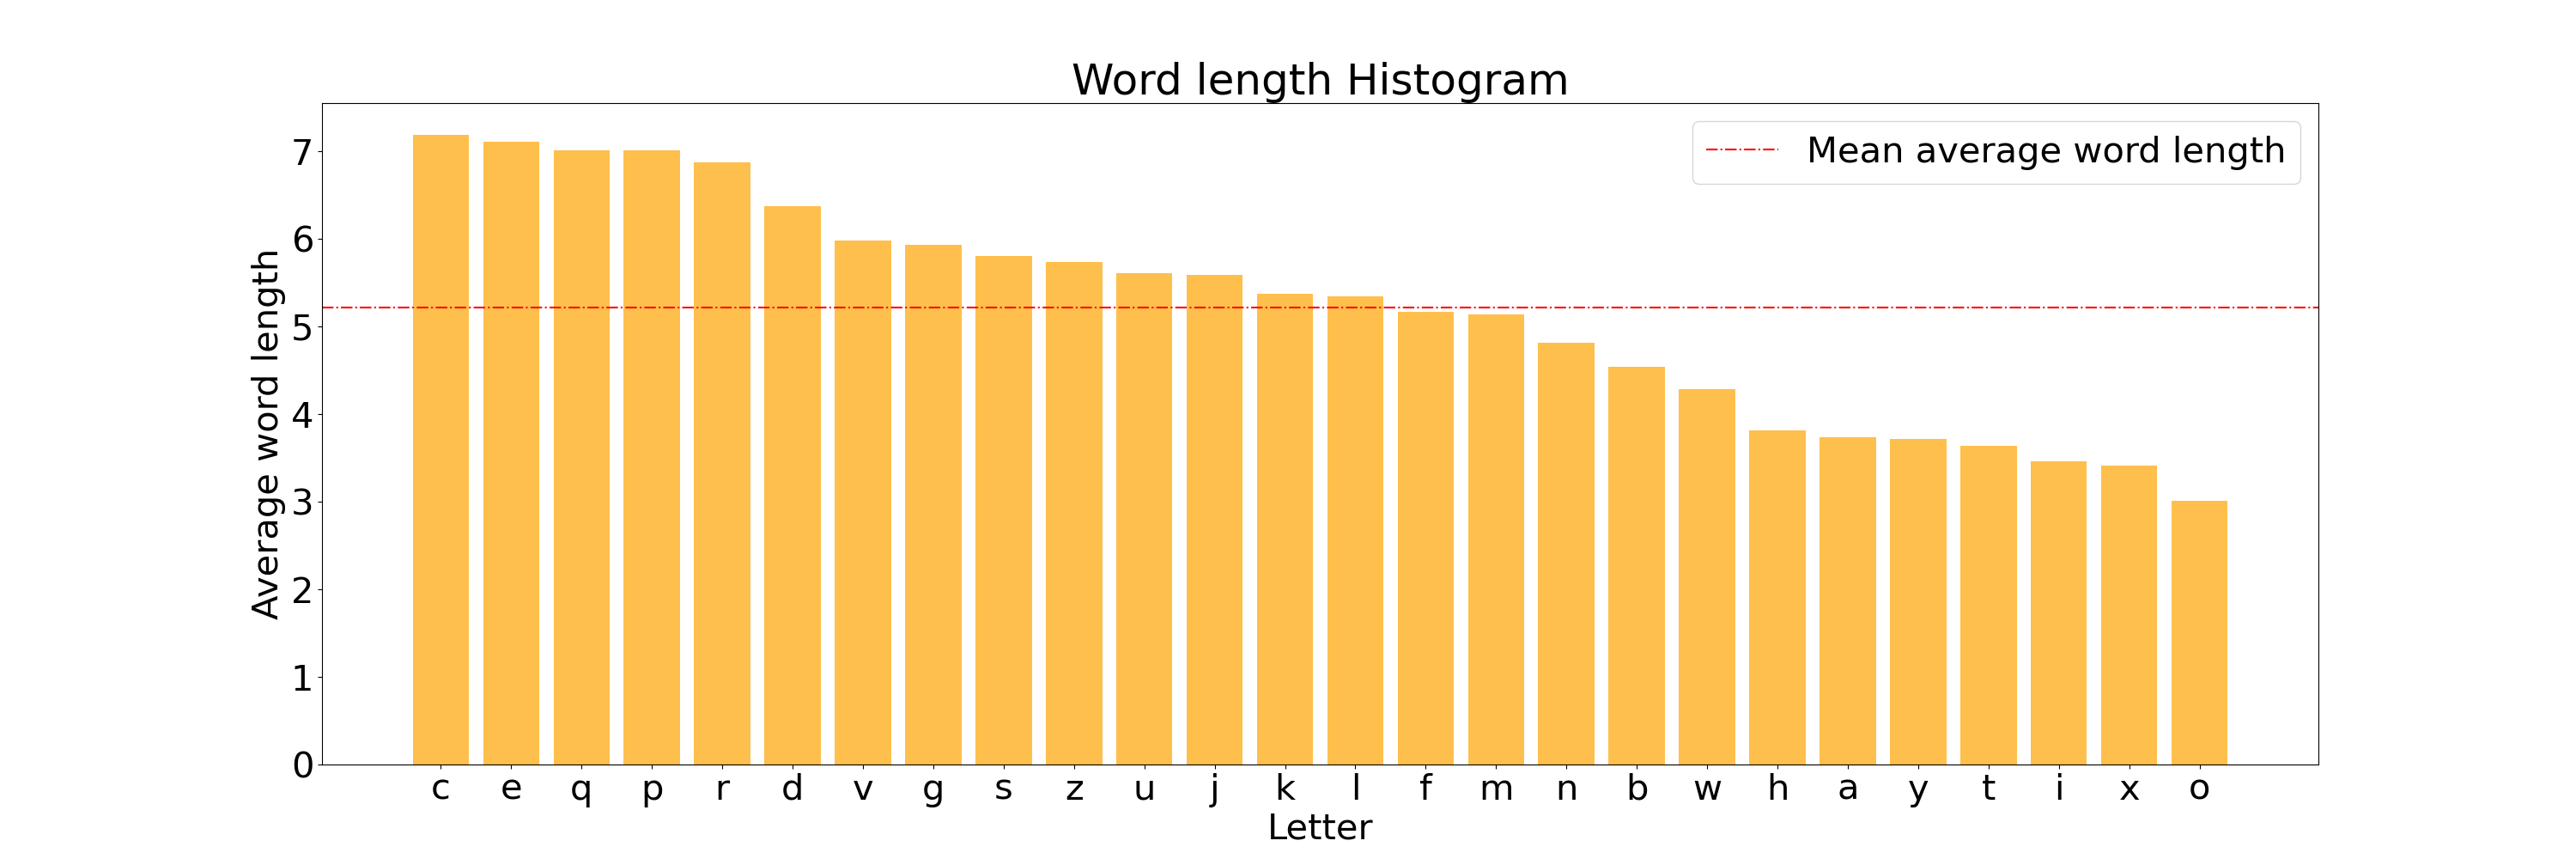
\includegraphics[width=\linewidth]{figures/download}
    \caption{A histogram depicting the average word length (y-axis) for every letter of the Latin alphabet (x-axis). The mean average length is shown as a horizontal red dashed line.}
    \label{img:histogram:word_lengths}
  \end{figure}
  

  \subsubsection{Evaluation}
  The experiments were executed using the dataset \texttt{SherlockHolmes.txt}. The results are listed below in a 10-column format and graphically depicted in~\autoref{img:histogram:word_lengths}.

  \begin{multicols}{10}
    \noindent
    c:7.19
    \\ e: 7.11
    \\ q: 7.01
    \\ p: 7.01
    \\ r: 6.87
    \\ d: 6.37
    \\ v: 5.98
    \\ g: 5.93
    \\ s: 5.8
    \\ z: 5.74
    \\ u: 5.61
    \\ j: 5.59
    \\ k: 5.37
    \\ l: 5.34
    \\ f: 5.17
    \\ m: 5.14
    \\ n: 4.81
    \\ b: 4.54
    \\ w: 4.28
    \\ h: 3.81
    \\ a: 3.74
    \\ y: 3.72
    \\ t: 3.64
    \\ i: 3.46
    \\ x: 3.41
    \\ o: 3.01
    \label{multicol:test}
  \end{multicols}

  \newpage
  \section{Problem 2: Airline Tweets analytics}
  \label{sec:problem2}
  The second problem focuses on producing analytic insights from an Twitter feedback post for airline services.


  \subsection{Problem Statement}
  In this task, we take on the role of a data analyst aiming to help airlines improve the quality of their services. Our data source is a CSV file (each row corresponds to a tweet) containing Twitter comments about airline services, with the following format:

  \begin{itemize}
    \item \texttt{tweet\_id}
    \item \texttt{airline\_sentiment}
    \item \texttt{airline\_sentiment\_confidence}
    \item \texttt{negativereason}
    \item \texttt{negativereason\_confidence}
    \item \texttt{airline}
    \item \texttt{name}
    \item \texttt{text}
    \item \texttt{tweet\_created}
    \item \texttt{user\_timezone}
  \end{itemize}

  You are required to create a program using Spark DataFrames to answer the following questions:

  \begin{enumerate}
    \item \textbf{What are the 5 words in the tweet text that appear most frequently for each \texttt{airline\_sentiment} category: positive, negative, and neutral?}
    \item \textbf{What is the main reason for complaint (\texttt{negativereason}) for each airline, i.e., the reason associated with the most tweets?} Consider only tweets with \texttt{negativereason\_confidence > 0.5}.
  \end{enumerate}

  In the implementation, you should ignore punctuation marks, and consider all words to be in lowercase for the related processing.

  \subsection{Proposed approach}
  \subsubsection{Setting}
  Our implementation is run and tested in a Linux environment with 12 cores, using the Scala programming language version 2.13.15 and Apache Spark version 3.5.3. We have used SBT as the build tool of our solution.
  We have used the Software Development Kit (JDK) version 11.0.11.
  The source code is developed in IntelliJ IDEA Community Edition 2021.1.1 and managed using SBT as the build tool. All dependencies of the project can be found in the \texttt{build.sbt} file located at the root folder of the project.
  The project is compiled and executed directly from the IntelliJ IDEA.

  To run the project, open the \texttt{src/main/scala/Task2AirlineTweets.scala} file in IntelliJ IDEA, and execute the main method. After successful execution of the program, the results can be viewed under the \texttt{output/task2} directory.

  \subsubsection{Implementation}
  The implementation utilizes Apache Spark for distributed processing, ensuring scalability for large datasets. The process is divided into two main tasks, described in detail below.
  \\

  \textit{Task 1: Extracting Top Words by Sentiment}
  \\

  \textbf{Preprocessing:}
  \begin{enumerate}
    \item Text was converted to lowercase to ensure case insensitivity.
    \item Non-alphabetic characters were removed using regular expressions, eliminating punctuation and special symbols.
  \end{enumerate}

  \textbf{Word Frequency Analysis:}
  \begin{enumerate}
    \item Tweets were filtered based on their sentiment (\texttt{airline\_sentiment} = positive, negative, or neutral).
    \item Tokenization was performed to split the cleaned text into individual words.
    \item A word frequency distribution was computed by grouping words and counting their occurrences.
    \item The top 5 most frequent words for each sentiment category were extracted and ranked.
  \end{enumerate}

  \textbf{Output:}
  Results were saved in separate directories (\texttt{output/task2/\{sentiment\}-top-words}) for each sentiment category as CSV files.
  \\

  \textit{Task 2: Identifying Main Complaint Reasons}
  \\

  \textbf{Filtering:}
  \begin{enumerate}
    \item Tweets with a non-null \texttt{negativereason} field were selected.
    \item Only tweets with \texttt{negativereason\_confidence} > 0.5 were considered to ensure reliable complaint reasons.
  \end{enumerate}

  \textbf{Grouping and Ranking:}
  \begin{enumerate}
    \item Tweets were grouped by \texttt{airline} and \texttt{negativereason}.
    \item The frequency of each complaint reason was calculated for each airline.
    \item A ranking function (\texttt{row\_number}) was applied within each airline's group to identify the most frequent complaint reason.
  \end{enumerate}

  \textbf{Output:}
  The results, including the airline, top complaint reason, and its frequency, were saved in a CSV file (\texttt{output/task2/top-complaints}).

  \paragraph{Implementation Details}
  The implementation uses the following key components of Apache Spark:
  \begin{itemize}
    \item \textbf{SparkSession:} Initializes the Spark application and provides the entry point for DataFrame operations.
    \item \textbf{DataFrame API:} Used for transformations, including filtering, grouping, and ranking.
    \item \textbf{Regular Expressions:} Applied to clean the text data by removing non-alphabetic characters.
    \item \textbf{Window Functions:} Enabled ranking of complaint reasons for each airline.
  \end{itemize}



  \subsubsection{Evaluation} Our solution is tested using the provided tweets dataset, namely \texttt{tweets.csv}. The results for each analytical query are presented below.

  \begin{table}[h!]
    \centering
    \begin{minipage}{0.30\textwidth}
      \centering
      \begin{tabular}{|c|c|}
        \hline
        \textbf{Word} & \textbf{Count} \\ \hline
        the & 903 \\ \hline
        to & 880 \\ \hline
        you & 811 \\ \hline
        for & 628 \\ \hline
        thanks & 587 \\ \hline
      \end{tabular}
      \caption{Top-5 positive words}
    \end{minipage} \hspace{0.3cm}
    \begin{minipage}{0.30\textwidth}
      \centering
      \begin{tabular}{|c|c|}
        \hline
        \textbf{Word} & \textbf{Count} \\ \hline
        to & 1573 \\ \hline
        i & 1126 \\ \hline
        the & 927 \\ \hline
        a & 774 \\ \hline
        united & 700 \\ \hline
      \end{tabular}
      \caption{Top-5 neutral words}
    \end{minipage}
    \begin{minipage}{0.30\textwidth}
      \centering
      \begin{tabular}{|c|c|}
        \hline
        \textbf{Word} & \textbf{Count} \\ \hline
        to & 5686 \\ \hline
        the & 3914 \\ \hline
        i & 3396 \\ \hline
        a & 3033 \\ \hline
        flight &2763 \\ \hline
      \end{tabular}
      \caption{Top-5 negative words}
    \end{minipage}
  \end{table}

  \begin{table}[h!]
    \centering
    \begin{tabular}{|c|c|c|}
      \hline
      \textbf{Airline} & \textbf{Reason} & \textbf{Count} \\ \hline
      American & Customer Service Issue & 654  \\ \hline
      Delta & Late Flight & 228 \\ \hline
      Southwest & Customer Service Issue & 323 \\ \hline
      US Airways & Customer Service Issue & 698 \\ \hline
      United & Customer Service Issue & 545 \\ \hline
      Virgin America & Customer Service Issue & 51 \\ \hline
    \end{tabular}
    \caption{Top complaints for each Airline}
  \end{table}


  \section{Problem 3: Movie Analytics}
  \label{sec:problem3}
  The third problem focuses on producing analytic insights into a movies dataset.


  \subsection{Problem Statement}
  In this problem, you are provided with a dataset that contains information about movies. Each record represents a movie and includes three main columns (attributes), namely \texttt{movieId}, \texttt{title} and \texttt{genres}. An example record of the dataset is the following:

  \begin{verbatim}
1,Toy Story (1995),Adventure|Animation|Children|Comedy|Fantasy
  \end{verbatim}

  Note that a movie can belong to multiple genres (e.g., adventure, fantasy, and so on). The genres are separated by a vertical line (`|') in the respective field. Your Apache Spark (Scala) application should compute the following analytics:
  \begin{enumerate}
    \item \textbf{How many movies are there for each genre?} If a movie belongs to multiple genres, it should be counted to all these genres. Sort the results by the name of genre in alphabetical order.
    \item \textbf{How many movies have been filmed per year?} Note that the year a movie was filmed is currently encoded into a composite movie title, e.g., ``\texttt{Toy Story (1995)}''. Show the top 10 years with the most movies filmed within them.
    \item \textbf{Which are the words that appear at least 10 times in the titles of the movies, and what is their total frequency?} You can ignore words that have less than 4 characters. Sort the results, showing first the words with the higher frequency.
  \end{enumerate}

  \subsection{Proposed approach}
  \subsubsection{Setting}
  Our implementation is run and tested in a Linux environment with 12 cores, using the Scala programming language version 2.13.15 and Apache Spark version 3.5.3. We have used SBT as the build tool of our solution.
  We have used the Software Development Kit (JDK) version 11.0.11.
  The source code is developed in IntelliJ IDEA Community Edition 2021.1.1 and managed using SBT as the build tool. All dependencies of the project can be found in the \texttt{build.sbt} file located at the root folder of the project.
  The project is compiled and executed directly from the IntelliJ IDEA.

  To run the project, open the \texttt{src/main/scala/Task3MovieAnalytics.scala} file in IntelliJ IDEA, and execute the main method. After successful execution of the program, the results can be viewed under the \texttt{output/task3} directory.

  \subsubsection{Implementation} We leverage Apache Spark \emph{DataFrames} API to calculate the aforementioned analytical queries. Our proposed approach comprises the following four stages:
  \begin{description}
    \item[Stage 1:] Data cleaning and preprocessing
    \item[Stage 2:] Computation of genre analytics (query 1)
    \item[Stage 3:] Computation of year analytics (query 2)
    \item[Stage 4:] Computation of title analytics (query 3)
  \end{description}
  \autoref{img:movieAnalyticsSolutionDiagram} graphically depicts the four stages, as well as their assembly in a workflow. We elaborate on each stage separately in the rest of the Subsection.

  \begin{figure}[tb!]
    \centering
    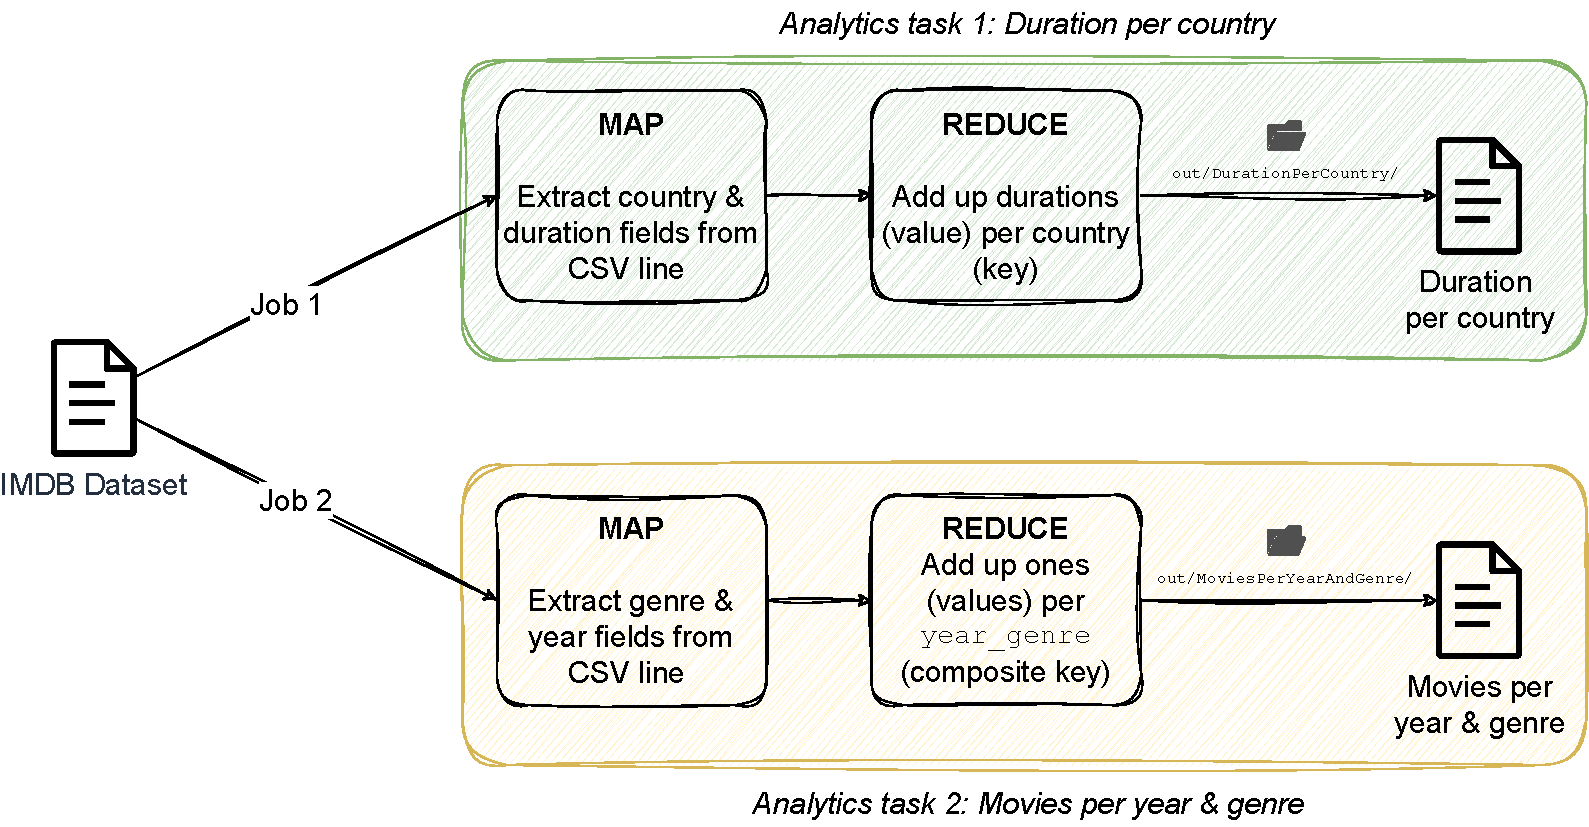
\includegraphics[width=0.7\linewidth]{figures/movieAnalytics}
    \caption{The four stages of our proposed approach to compute the movie analytics, assembled in a workflow.}
    \label{img:movieAnalyticsSolutionDiagram}
  \end{figure}

  \paragraph{Stage1: Data Cleaning and preprocessing} In this stage, we address data quality issues that are present in the raw movie data. Missing production year, missing genres and trailing whitespaces in the title string are the detected data quality issues. To address these issues, we explicitly mark the movie year as ``N/A'' (not available) \& movie genre as ``(no genre listed)'' and trim the composite title strings, respectively. Subsequently, we transform the data representation to a more efficient form, by extracting the actual title and year to separate fields (instead of a composite one) and splitting the genres composite string field to an array of genres. Throughout the whole process, we \textbf{use solely the DataFrame API} of Apache Spark, leveraging also the pattern matching functionality of Scala. A small sample of the cleaned and transformed DataFrame shown in~\autoref{img:movieAnalyticsSolutionDiagram} is depicted below:

  \begin{verbatim}
                  +-------+--------------------+--------------------+----+
                  |movieId|               title|              genres|year|
                  +-------+--------------------+--------------------+----+
                  |      1|           Toy Story|[Adventure, Anima...|1995|
                  |      2|             Jumanji|[Adventure, Child...|1995|
                  |      3|    Grumpier Old Men|   [Comedy, Romance]|1995|
                  |      4|   Waiting to Exhale|[Comedy, Drama, R...|1995|
                  |      5|Father of the Bri...|            [Comedy]|1995|
                  +-------+--------------------+--------------------+----+
  \end{verbatim}

  \paragraph{Stage 2: Computation of genre analytics} In this stage, we use the cleaned and transformed data to compute analytical insights into the movie genres. In particular, we use the DataFrame API (\texttt{select()}, \texttt{group\_by()}, etc.) to calculate the number of movies that belong to each genre. An implementation detail of our solution lies in handling the cases where a movie belongs to multiple genres. To ensure the integrity of the computed analytics, we opt for using the \texttt{explode()} function of the DataFrame API, to transform the array of genres to separate genre items. The analytics are, then, computed on top of this extra transformation, enabling us to \textbf{include a movie into the calculations of all the genres it belongs}.

  \paragraph{Stage 3: Computation of year analytics} In this stage, we use the cleaned and transformed data to compute analytical insights into the movie production years. Similarly to Stage 2, we leverage exclusively the DataFrame API to calculate the total number of movies filmed each year. In this case, the \texttt{group\_by} operation is more straightforward, since the cleaned and transformed DataFrame contains a dedicated column for the movie production year.

  \paragraph{Stage 4: Computation of title analytics} Similarly to Stage 2, we use operations available from the DataFrame API to calculate the most frequently used words in the movie titles. We, leverage the \texttt{split(" ")} and \texttt{explode()} functions to transform titles, first, into an array of words and, then, into separate words that are finally grouped and aggregated. We remove words that have less than 4 characters and fundamental stopwords, such as ``with'', or ``from'', in order to obtain analytical insights of high quality.

  \subsubsection{Evaluation} Our solution is tested using the raw movie data, namely \texttt{movies.csv}. We list the execution results below, if of appropriate length, else in~\autoref{sec:data3}.

  \paragraph{Stage 2: Computation of genre analytics}
  We list here the execution results for the genre analytics query in a 6-column format.
  \begin{multicols}{6}
    \noindent
    Action: 7348
    \\ Adventure: 4145
    \\ Animation: 2929
    \\ Children: 2935
    \\ Comedy: 16870
    \\ Crime: 5319
    \\ Documentary: 5605
    \\ Drama: 25606
    \\ Fantasy: 2731
    \\ Film-Noir: 353
    \\ Horror: 5989
    \\ IMAX: 195
    \\ Musical: 1054
    \\ Mystery: 2925
    \\ Romance: 7719
    \\ Sci-Fi: 3595
    \\ Thriller: 8654
    \\ War: 1874
    \\ Western: 1399
    \\ N/A: 5062
  \end{multicols}

  \paragraph{Stage 3: Computation of year analytics}
  We list here the execution results for the year analytics query in a 3-column format, i.e., the top 10 years with the most movies. We observe that these years span the time period between 2009 and 2018, excluding 2015, indicating a heavy film production process in this decade. \autoref{img:movies_per_year} depicts the distribution of movies per year for all years in chronological order. Our findings indicate a clear long-tail distribution of movies over the years, with a burst of new movies over the last decade.
  \begin{multicols}{3}
    \centering
    \noindent
    2015: 2512 movies
    \\ 2016: 2488 movies
    \\ 2014: 2406 movies
    \\ 2017: 2373 movies
    \\ 2013: 2173 movies
    \\ 2018: 2032 movies
    \\ 2012: 1978 movies
    \\ 2011: 1838 movies
    \\ 2009: 1724 movies
    \\ 2010: 1691 movies
  \end{multicols}

  \begin{figure}[tb!]
    \centering
    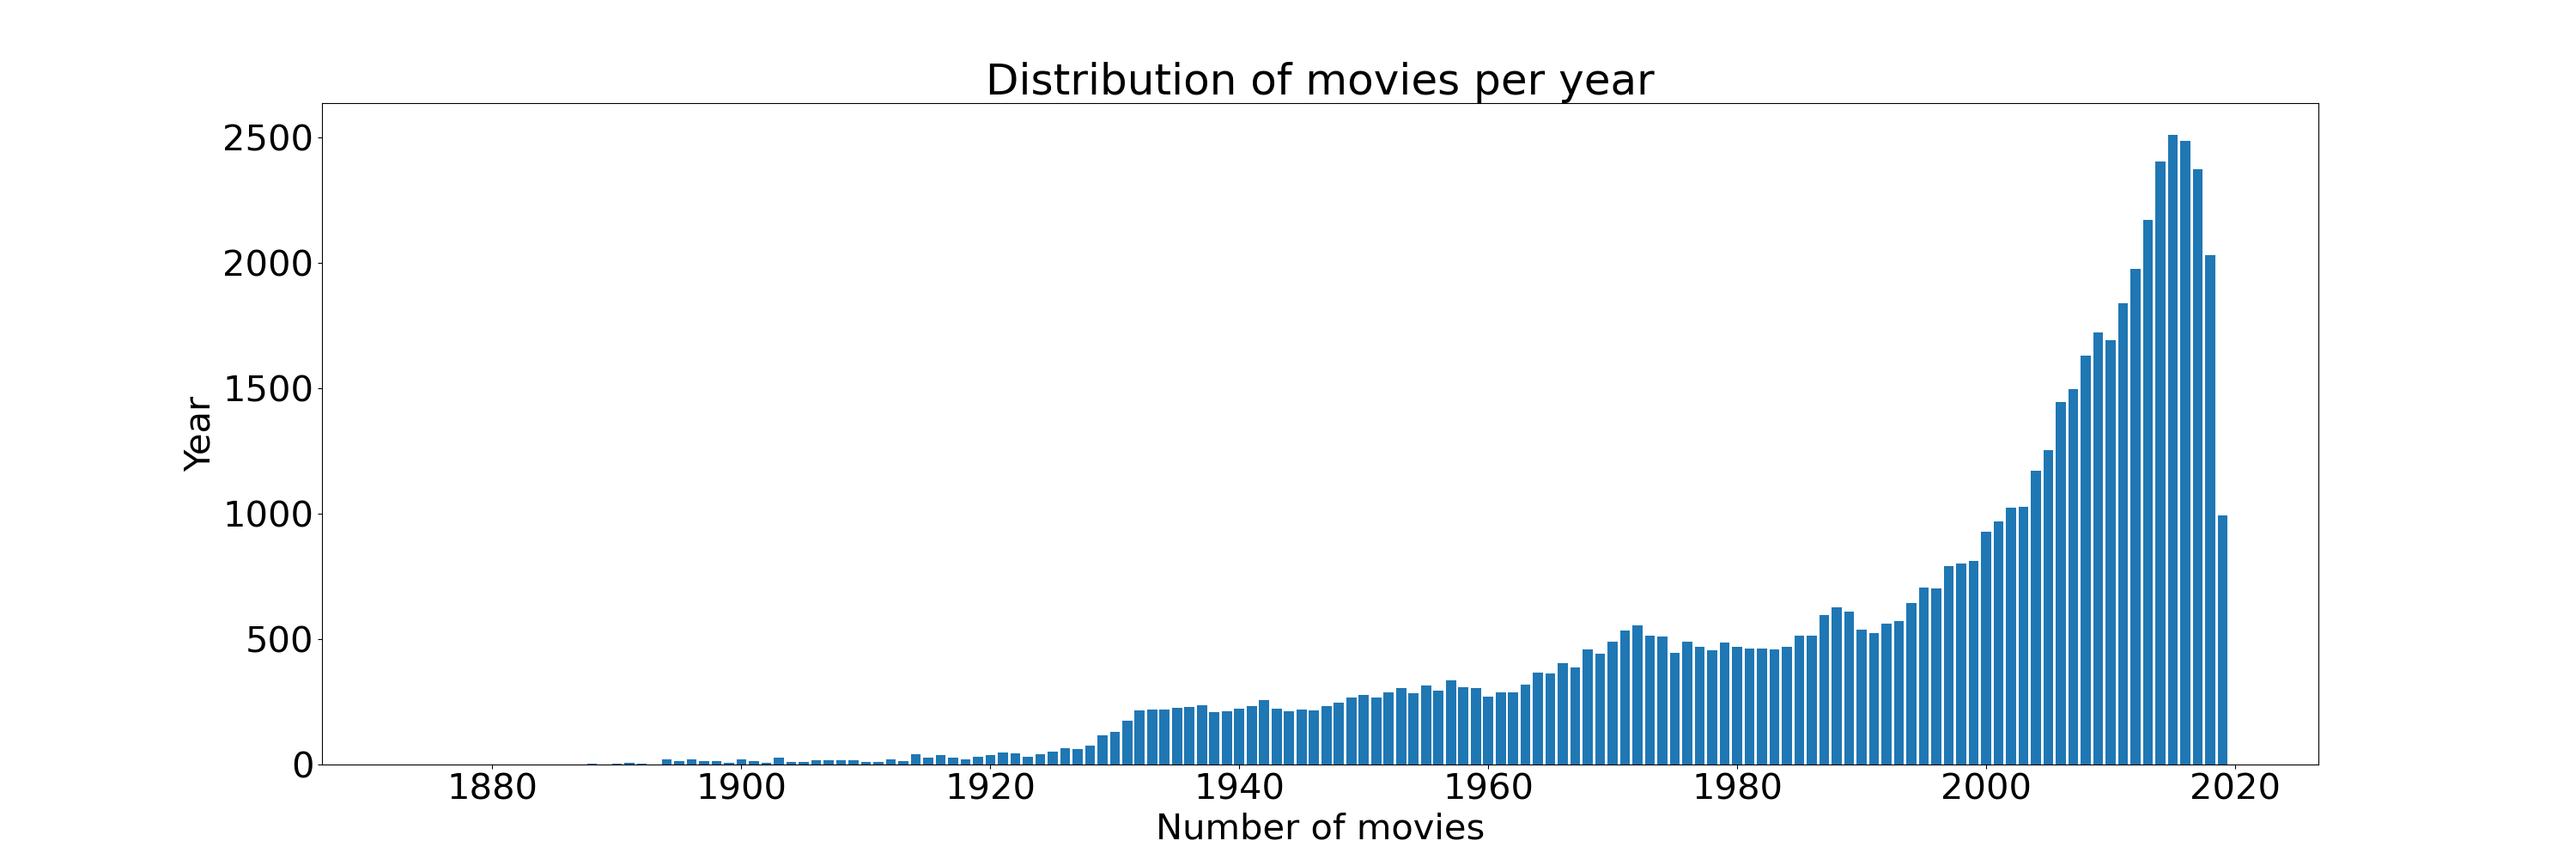
\includegraphics[width=\linewidth]{figures/movies per year}
    \caption{The distribution of the total number of movies per year in the dataset used for evaluating our solution.}
    \label{img:movies_per_year}
  \end{figure}

  \paragraph{Stage 4: Computation of title analytics}
  We list in~\autoref{sec:data3} the execution results for the title analytics query. Also, ~\autoref{img:word_cloud} depicts a word cloud with the most frequently used words in movie titles, found in the dataset used for evaluating our solution. Note that the bigger a word is, the more frequently it appears in movie titles.
  \begin{figure}[tb!]
    \centering
    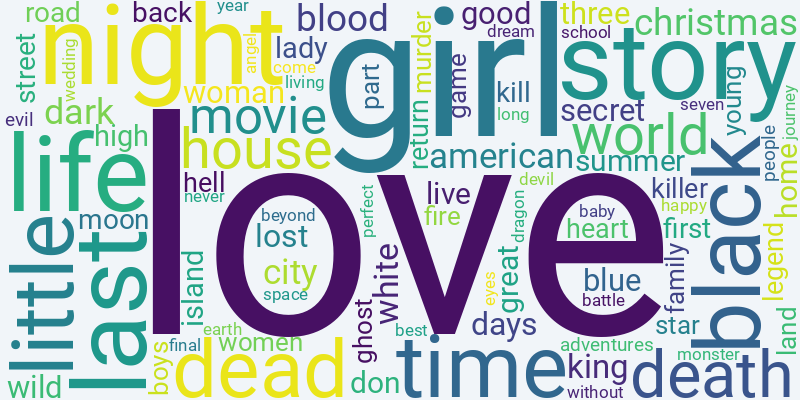
\includegraphics[width=0.8\linewidth]{figures/word cloud}
    \caption{A word cloud depicting the most frequent words appearing in the titles of the movies in the dataset examined. The bigger a word is, the more frequently it appears in the titles of the movies.}
    \label{img:word_cloud}
  \end{figure}

  \section{Problem 4: Probabilistic graph}
  \label{sec:problem4}
  We discuss here the fourth problem of the assignment.
  The main target of the assignment is to get acquainted with performing various MapReduce phases on a pipeline frame.

  \subsection{Problem Statement}
  Given a directed graph consisting of nodes and directed edges, stored in the edge-list format in a txt or csv file, you are requested to do the following tasks:
  \begin{itemize}
    \item Implement a program, utilizing the RDD Spark's framework, that for each node of the graph, it will calculate the number of incoming and the number of outgoing edges. The program should print out the 10 nodes with the most incoming and outgoing edges, respectively.
    \item Modify the previous implementation, so as not to discriminate the direction of the edge, so that the degree of a node is calculated by the number of edges lying on it. The program should print the number of nodes with degree greater than or equal to the mean degree.
  \end{itemize}
  Use the edge-list (txt) file provided in \url{http://snap.stanford.edu/data/web-Stanford.txt.gz}.
  \begin{figure}[h]
    \centering
    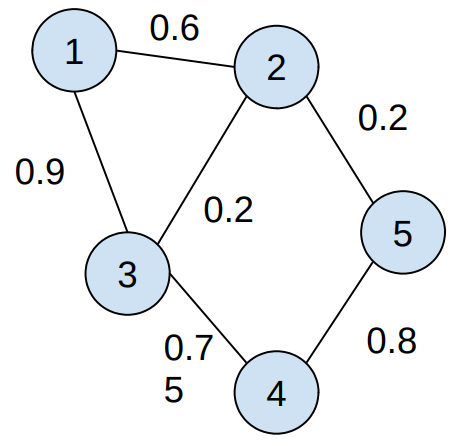
\includegraphics[width=0.25\linewidth]{figures/graph}
  \end{figure}

  \subsection{Proposed approach}
  \subsubsection{Setting}
  Our implementation is run and tested in a Linux environment with 12 cores, using the Scala programming language version 2.13.15 and Apache Spark version 3.5.3. We have used SBT as the build tool of our solution.
  We have used the Software Development Kit (JDK) version 11.0.11.
  The source code is developed in IntelliJ IDEA Community Edition 2021.1.1 and managed using SBT as the build tool. All dependencies of the project can be found in the \texttt{build.sbt} file located at the root folder of the project.
  The project is compiled and executed directly from the IntelliJ IDEA.

  To run the project, open the \texttt{src/main/scala/Task4GraphEdgeCounts.scala} file in IntelliJ IDEA, and execute the main method. After successful execution of the program, the results can be viewed under the \texttt{output/task4} directory.


  \subsubsection{Implementation}
  The task involves working with a directed graph stored in an edge-list format, where each edge is represented as a tuple of source and destination nodes. The goal is to develop a solution using Apache Spark's Resilient Distributed Datasets (RDDs) framework to calculate and analyze edge counts for the nodes in the graph. The approach consists of the following key steps:

  \textbf{Preprocessing.}
  First, the graph data, stored in a text or CSV file, is read into an RDD. The RDD is filtered to remove any comments (lines starting with \texttt{\#}), ensuring that only valid edge data is processed.

  For each edge in the graph, the source node is identified, and a tuple \texttt{(src, 1)} is created for each source node. These tuples (\texttt{outgoingCounts}) are then aggregated by the \texttt{reduceByKey} function to calculate the total number of outgoing edges for each node. The result is an RDD of node and outgoing edge count pairs.

  Similarly, for each edge, the destination node is identified, and a tuple \texttt{(dest, 1)} is created for each destination node. The \texttt{reduceByKey} function is again used to calculate the total number of incoming edges for each node,    resulting in an RDD of node and incoming edge count pairs (\texttt{incomingCounts}).

  \textbf{Top 10 nodes}
  To identify the top 10 nodes with the most incoming and outgoing edges, the \texttt{top} function is used, which sorts the nodes in descending order based on the edge counts. These top nodes are saved into separate output files: one for the nodes with the most incoming edges and another for the nodes with the most outgoing edges.

  \textbf{Degree-based filtering}
  In the modified implementation, the direction of the edges is ignored to calculate the degree of each node. The degree is calculated as the sum of the incoming and outgoing edge counts for each node. This is achieved using a \texttt{fullOuterJoin} between the RDDs of incoming and outgoing edge counts, followed by a transformation that sums the values for each node. In cases where a node only has outgoing or incoming edges but not both, the missing values are treated as 0.

  The mean degree of the graph is then calculated by summing the degrees of all nodes and dividing by the total number of nodes. This value is used to filter the nodes with a degree greater than or equal to the mean degree.

  The filtered nodes are saved to an output file, and the total count of such nodes is printed. This provides insight into how many nodes in the graph have a degree that meets or exceeds the average.

  The final output consists of the following:
  \begin{itemize}
    \item The 10 nodes with the most incoming edges.
    \item The 10 nodes with the most outgoing edges.
    \item The number of nodes with a degree greater than or equal to the mean degree, along with the corresponding list of nodes.
  \end{itemize}

  \subsubsection{Evaluation} Our solution is tested using the provided edge-list Stanford dataset, namely \texttt{web-Stanford.txt}. The results are presented below.

  \begin{table}[h!]
    \centering
    \begin{minipage}{0.45\textwidth}
      \centering
      \begin{tabular}{|c|c|}
        \hline
        \textbf{Node} & \textbf{Incoming} \\ \hline
        226411 & 38606\\ \hline
        234704 & 21920\\ \hline
        105607 & 19457\\ \hline
        241454 & 19377\\ \hline
        167295  & 19003\\ \hline
        198090 & 18975\\ \hline
        81435 & 18970\\ \hline
        214128 & 18967\\ \hline
        38342 & 18958\\ \hline
        245659 & 18935\\ \hline
      \end{tabular}
      \caption{Top-10 nodes with most incoming edges}
    \end{minipage} \hspace{0.3cm}
    \begin{minipage}{0.45\textwidth}
      \centering
      \begin{tabular}{|c|c|}
        \hline
        \textbf{Node} & \textbf{Incoming} \\ \hline
        82409 & 255\\ \hline
        82868 & 247\\ \hline
        188978 & 247\\ \hline
        16984 & 247\\ \hline
        86290 & 247\\ \hline
        180611 & 247\\ \hline
        10699 & 245\\ \hline
        121634 & 245\\ \hline
        176419 & 244\\ \hline
        255711 & 244\\ \hline
      \end{tabular}
      \caption{Top-10 nodes with most outgoing edges}
    \end{minipage}
  \end{table}

  \begin{table}[h!]
    \centering
    \begin{tabular}{|c|c|c|}
      \hline
      \textbf{Airline} & \textbf{Reason} & \textbf{Count} \\ \hline
      American & Customer Service Issue & 654  \\ \hline
      Delta & Late Flight & 228 \\ \hline
      Southwest & Customer Service Issue & 323 \\ \hline
      US Airways & Customer Service Issue & 698 \\ \hline
      United & Customer Service Issue & 545 \\ \hline
      Virgin America & Customer Service Issue & 51 \\ \hline
    \end{tabular}
    \caption{Top complaints for each Airline}
  \end{table}

  The number of nodes with degree greater than or equal to the average degree (16.41) is \textbf{54933}.

  \section{Conclusion}
  \label{sec:conclusion}
  In this document we have presented our solutions and rationale for solving the second assignment of the M.Sc.
  course on \emph{Technologies for Big Data Analysis}, offered by the \emph{DWS M.Sc. Program}. For each one of the four problems of the assignment, we have presented their statement, as well as the solution approach we have adopted. All execution results with the provided datasets can be found in the appendices of our work.

  \newpage
  \appendix

  \section{Problem 3 execution results}
  \label{sec:data3}
  \begin{multicols}{6}
  % \centering
  \noindent
  love: 851
  \\ night: 519
  \\ story: 495
  \\ life: 476
  \\ last: 451
  \\ girl: 387
  \\ black: 352
  \\ time: 350
  \\ little: 335
  \\ dead: 327
  \\ death: 323
  \\ house: 311
  \\ world: 306
  \\ movie: 286
  \\ christmas: 274
  \\ blood: 271
  \\ dark: 258
  \\ city: 250
  \\ american: 249
  \\ white: 235
  \\ your: 225
  \\ king: 219
  \\ lost: 209
  \\ days: 209
  \\ secret: 202
  \\ that: 201
  \\ blue: 200
  \\ woman: 197
  \\ good: 196
  \\ three: 194
  \\ wild: 192
  \\ summer: 185
  \\ great: 181
  \\ home: 181
  \\ girls: 180
  \\ don't: 179
  \\ live: 179
  \\ lady: 169
  \\ island: 168
  \\ high: 166
  \\ this: 165
  \\ road: 159
  \\ back: 158
  \\ what: 156
  \\ kill: 156
  \\ street: 155
  \\ moon: 154
  \\ first: 153
  \\ about: 152
  \\ the): 147
  \\ hell: 146
  \\ legend: 146
  \\ killer: 145
  \\ heart: 145
  \\ return: 144
  \\ when: 142
  \\ like: 142
  \\ young: 139
  \\ ghost: 138
  \\ family: 137
  \\ star: 137
  \\ women: 135
  \\ part: 135
  \\ boys: 134
  \\ game: 133
  \\ murder: 129
  \\ land: 129
  \\ fire: 125
  \\ adventures: 121
  \\ people: 121
  \\ under: 120
  \\ after: 117
  \\ evil: 116
  \\ down: 114
  \\ journey: 114
  \\ never: 114
  \\ beyond: 113
  \\ devil: 112
  \\ perfect: 111
  \\ living: 111
  \\ long: 110
  \\ space: 108
  \\ monster: 108
  \\ wedding: 108
  \\ school: 108
  \\ best: 108
  \\ year: 107
  \\ battle: 106
  \\ final: 106
  \\ baby: 106
  \\ come: 106
  \\ angel: 105
  \\ eyes: 104
  \\ happy: 103
  \\ before: 102
  \\ earth: 101
  \\ without: 101
  \\ dragon: 101
  \\ dream: 101
  \\ seven: 100
  \\ kiss: 99
  \\ room: 99
  \\ magic: 99
  \\ it's: 98
  \\ party: 98
  \\ just: 98
  \\ town: 98
  \\ children: 98
  \\ man,: 98
  \\ will: 97
  \\ four: 97
  \\ tale: 97
  \\ heaven: 97
  \\ other: 95
  \\ river: 95
  \\ fear: 95
  \\ over: 95
  \\ they: 94
  \\ here: 94
  \\ golden: 93
  \\ sweet: 93
  \\ five: 93
  \\ years: 92
  \\ beautiful: 92
  \\ film: 91
  \\ west: 91
  \\ case: 91
  \\ green: 90
  \\ crazy: 88
  \\ water: 88
  \\ once: 88
  \\ fall: 87
  \\ song: 87
  \\ wolf: 86
  \\ paris: 85
  \\ deadly: 85
  \\ queen: 85
  \\ america: 84
  \\ miss: 84
  \\ true: 84
  \\ midnight: 84
  \\ into: 83
  \\ hero: 83
  \\ snow: 82
  \\ dance: 81
  \\ light: 81
  \\ jack: 81
  \\ hard: 81
  \\ goes: 81
  \\ hollywood: 80
  \\ only: 79
  \\ princess: 79
  \\ rock: 79
  \\ another: 79
  \\ dreams: 78
  \\ prince: 78
  \\ angels: 78
  \\ john: 77
  \\ escape: 77
  \\ terror: 77
  \\ cold: 77
  \\ shadow: 77
  \\ zero: 76
  \\ brothers: 76
  \\ call: 76
  \\ strange: 76
  \\ take: 75
  \\ inside: 75
  \\ money: 74
  \\ iron: 74
  \\ charlie: 74
  \\ country: 74
  \\ wind: 74
  \\ side: 74
  \\ wife: 73
  \\ mystery: 73
  \\ paradise: 73
  \\ tales: 73
  \\ where: 73
  \\ bride: 73
  \\ father: 72
  \\ again: 72
  \\ gold: 72
  \\ mountain: 71
  \\ truth: 71
  \\ revenge: 71
  \\ book: 71
  \\ beast: 69
  \\ face: 69
  \\ lucky: 69
  \\ adventure: 69
  \\ edge: 69
  \\ york: 69
  \\ deep: 69
  \\ hotel: 68
  \\ devil's: 68
  \\ vampire: 68
  \\ stranger: 68
  \\ dawn: 68
  \\ child: 68
  \\ behind: 68
  \\ name: 67
  \\ mother: 67
  \\ dangerous: 67
  \\ planet: 67
  \\ trouble: 67
  \\ born: 67
  \\ crime: 66
  \\ special: 66
  \\ there: 66
  \\ winter: 66
  \\ park: 66
  \\ blues: 66
  \\ human: 66
  \\ lives: 66
  \\ lake: 66
  \\ meet: 66
  \\ north: 66
  \\ friends: 65
  \\ beach: 65
  \\ silent: 65
  \\ free: 65
  \\ next: 65
  \\ times: 65
  \\ captain: 65
  \\ have: 65
  \\ jungle: 65
  \\ tomorrow: 64
  \\ forever: 64
  \\ dirty: 64
  \\ detective: 64
  \\ away: 64
  \\ curse: 64
  \\ alien: 64
  \\ body: 63
  \\ train: 63
  \\ double: 63
  \\ private: 63
  \\ second: 63
  \\ alone: 63
  \\ darkness: 63
  \\ daughter: 62
  \\ diary: 62
  \\ nothing: 62
  \\ point: 62
  \\ beauty: 61
  \\ spring: 61
  \\ history: 61
  \\ broken: 61
  \\ were: 61
  \\ play: 61
  \\ nightmare: 60
  \\ comedy: 60
  \\ comes: 59
  \\ master: 59
  \\ place: 59
  \\ naked: 58
  \\ super: 58
  \\ johnny: 58
  \\ made: 58
  \\ killing: 58
  \\ show: 57
  \\ stars: 57
  \\ (les: 57
  \\ witch: 57
  \\ santa: 57
  \\ holiday: 57
  \\ rose: 57
  \\ still: 56
  \\ nights: 56
  \\ ride: 56
  \\ hill: 56
  \\ things: 56
  \\ flight: 56
  \\ upon: 56
  \\ fury: 56
  \\ rise: 55
  \\ rain: 55
  \\ garden: 55
  \\ club: 55
  \\ brother: 55
  \\ right: 55
  \\ know: 55
  \\ doctor: 55
  \\ valley: 54
  \\ phantom: 54
  \\ treasure: 54
  \\ machine: 54
  \\ zombie: 54
  \\ blind: 54
  \\ glory: 54
  \\ force: 54
  \\ horse: 53
  \\ power: 53
  \\ welcome: 53
  \\ castle: 53
  \\ head: 53
  \\ music: 53
  \\ massacre: 52
  \\ attack: 52
  \\ real: 52
  \\ camp: 52
  \\ going: 52
  \\ fight: 52
  \\ kids: 52
  \\ shadows: 52
  \\ affair: 52
  \\ miracle: 51
  \\ hunter: 51
  \\ flying: 51
  \\ soul: 51
  \\ small: 51
  \\ alive: 51
  \\ future: 50
  \\ heroes: 50
  \\ london: 50
  \\ dogs: 50
  \\ through: 50
  \\ something: 50
  \\ vengeance: 50
  \\ tiger: 50
  \\ operation: 49
  \\ more: 49
  \\ wars: 49
  \\ sunday: 49
  \\ mary: 49
  \\ flesh: 49
  \\ between: 49
  \\ gang: 49
  \\ secrets: 49
  \\ broadway: 49
  \\ china: 49
  \\ skin: 48
  \\ love,: 48
  \\ stone: 48
  \\ grace: 48
  \\ horror: 48
  \\ iii:: 48
  \\ invisible: 48
  \\ storm: 48
  \\ walk: 48
  \\ sword: 48
  \\ line: 48
  \\ mind: 48
  \\ friend: 47
  \\ mrs.: 47
  \\ samurai: 47
  \\ you're: 47
  \\ bill: 47
  \\ express: 47
  \\ against: 47
  \\ most: 47
  \\ came: 47
  \\ harry: 46
  \\ texas: 46
  \\ enemy: 46
  \\ hunt: 46
  \\ silence: 46
  \\ hearts: 46
  \\ ninja: 46
  \\ george: 46
  \\ company: 46
  \\ open: 46
  \\ stories: 46
  \\ haunted: 45
  \\ full: 45
  \\ desert: 45
  \\ lies: 44
  \\ tokyo: 44
  \\ always: 44
  \\ door: 44
  \\ mine: 44
  \\ les): 44
  \\ left: 44
  \\ project: 44
  \\ glass: 44
  \\ lovers: 44
  \\ make: 44
  \\ dear: 44
  \\ hour: 44
  \\ hands: 44
  \\ gone: 44
  \\ soldier: 44
  \\ very: 44
  \\ sister: 44
  \\ hope: 43
  \\ voyage: 43
  \\ david: 43
  \\ hidden: 43
  \\ alice: 43
  \\ dust: 43
  \\ grand: 43
  \\ louis: 43
  \\ demon: 43
  \\ missing: 43
  \\ mission: 43
  \\ rising: 43
  \\ guns: 43
  \\ state: 43
  \\ being: 43
  \\ romance: 43
  \\ making: 43
  \\ called: 43
  \\ trail: 42
  \\ wall: 42
  \\ thief: 42
  \\ code: 42
  \\ yellow: 42
  \\ tell: 42
  \\ than: 42
  \\ tree: 42
  \\ thing: 42
  \\ pink: 42
  \\ sisters: 42
  \\ holy: 42
  \\ story,: 42
  \\ sleep: 42
  \\ bloody: 42
  \\ killed: 42
  \\ can't: 41
  \\ forbidden: 41
  \\ bridge: 41
  \\ mars: 41
  \\ chapter: 41
  \\ morning: 41
  \\ class: 41
  \\ michael: 41
  \\ breaking: 41
  \\ warrior: 41
  \\ goodbye: 41
  \\ justice: 41
  \\ frankenstein: 41
  \\ kingdom: 40
  \\ faces: 40
  \\ touch: 40
  \\ heat: 40
  \\ anna: 40
  \\ fast: 40
  \\ kung: 40
  \\ late: 40
  \\ games: 40
  \\ teenage: 40
  \\ work: 40
  \\ dracula: 40
  \\ freedom: 40
  \\ vacation: 40
  \\ man's: 40
  \\ trip: 40
  \\ cool: 40
  \\ i'll: 39
  \\ must: 39
  \\ everything: 39
  \\ brave: 39
  \\ kind: 39
  \\ giant: 39
  \\ shark: 39
  \\ third: 39
  \\ want: 39
  \\ sound: 39
  \\ bird: 39
  \\ confessions: 39
  \\ honor: 39
  \\ monsters: 39
  \\ business: 39
  \\ fish: 39
  \\ lion: 38
  \\ passion: 38
  \\ portrait: 38
  \\ wrong: 38
  \\ youth: 38
  \\ across: 38
  \\ million: 38
  \\ every: 38
  \\ look: 38
  \\ chance: 38
  \\ running: 38
  \\ flower: 37
  \\ burning: 37
  \\ unknown: 37
  \\ savage: 37
  \\ bear: 37
  \\ date: 37
  \\ let's: 37
  \\ fever: 37
  \\ search: 37
  \\ forest: 37
  \\ sherlock: 37
  \\ life,: 37
  \\ funny: 37
  \\ pretty: 37
  \\ ever: 37
  \\ circle: 36
  \\ saint: 36
  \\ thunder: 36
  \\ revolution: 36
  \\ takes: 36
  \\ race: 36
  \\ cinderella: 36
  \\ minutes: 36
  \\ national: 36
  \\ police: 36
  \\ coming: 36
  \\ hours: 36
  \\ friday: 36
  \\ better: 36
  \\ walking: 36
  \\ gods: 36
  \\ lone: 36
  \\ wonderful: 36
  \\ brain: 36
  \\ thousand: 36
  \\ army: 35
  \\ above: 35
  \\ french: 35
  \\ royal: 35
  \\ wish: 35
  \\ jane: 35
  \\ short: 35
  \\ century: 35
  \\ quiet: 35
  \\ south: 35
  \\ within: 34
  \\ greatest: 34
  \\ agent: 34
  \\ hand: 34
  \\ woman,: 34
  \\ kings: 34
  \\ central: 34
  \\ beginning: 34
  \\ zombies: 34
  \\ season: 34
  \\ ghosts: 34
  \\ rage: 34
  \\ frank: 34
  \\ empire: 34
  \\ happiness: 34
  \\ billy: 34
  \\ hood: 34
  \\ easy: 34
  \\ legacy: 34
  \\ east: 34
  \\ half: 34
  \\ weekend: 34
  \\ bullet: 34
  \\ among: 33
  \\ blonde: 33
  \\ chasing: 33
  \\ spirit: 33
  \\ amazing: 33
  \\ hate: 33
  \\ silver: 33
  \\ married: 33
  \\ bang: 33
  \\ shoot: 33
  \\ souls: 33
  \\ around: 33
  \\ worlds: 33
  \\ shot: 33
  \\ number: 33
  \\ blade: 32
  \\ trial: 32
  \\ robin: 32
  \\ their: 32
  \\ madness: 32
  \\ ring: 32
  \\ paul: 32
  \\ richard: 32
  \\ looking: 32
  \\ lord: 32
  \\ carry: 32
  \\ beat: 32
  \\ some: 31
  \\ henry: 31
  \\ untold: 31
  \\ stand: 31
  \\ action: 31
  \\ berlin: 31
  \\ past: 31
  \\ tour: 31
  \\ lover: 31
  \\ wonder: 31
  \\ generation: 31
  \\ jesus: 31
  \\ them: 31
  \\ talk: 31
  \\ woods: 31
  \\ monkey: 31
  \\ brown: 31
  \\ movie:: 31
  \\ jimmy: 31
  \\ wanted: 31
  \\ strangers: 30
  \\ honey: 30
  \\ butterfly: 30
  \\ eagle: 30
  \\ marriage: 30
  \\ falling: 30
  \\ hills: 30
  \\ letter: 30
  \\ steel: 30
  \\ killers: 30
  \\ scooby-doo!: 30
  \\ perry: 30
  \\ wings: 30
  \\ public: 30
  \\ warriors: 30
  \\ break: 30
  \\ snake: 30
  \\ mark: 30
  \\ color: 30
  \\ dancing: 30
  \\ tears: 30
  \\ danger: 30
  \\ county: 30
  \\ lonely: 30
  \\ elephant: 30
  \\ keep: 30
  \\ almost: 30
  \\ flowers: 29
  \\ quest: 29
  \\ returns: 29
  \\ movie,: 29
  \\ meets: 29
  \\ guys: 29
  \\ circus: 29
  \\ manhattan: 29
  \\ world,: 29
  \\ sing: 29
  \\ nowhere: 29
  \\ band: 29
  \\ beneath: 29
  \\ remember: 29
  \\ finding: 29
  \\ rabbit: 29
  \\ musical: 29
  \\ lights: 29
  \\ nine: 29
  \\ getting: 29
  \\ picture: 29
  \\ gangster: 29
  \\ loves: 29
  \\ farm: 28
  \\ magnificent: 28
  \\ sleeping: 28
  \\ below: 28
  \\ chan: 28
  \\ happened: 28
  \\ belle: 28
  \\ roll: 28
  \\ merry: 28
  \\ doll: 28
  \\ ball: 28
  \\ you,: 28
  \\ chinese: 28
  \\ grave: 28
  \\ zone: 28
  \\ rome: 28
  \\ creek: 28
  \\ brooklyn: 28
  \\ wonderland: 28
  \\ waiting: 28
  \\ pirates: 28
  \\ della: 28
  \\ cinema: 28
  \\ jones: 28
  \\ those: 27
  \\ hercules: 27
  \\ falls: 27
  \\ holmes: 27
  \\ scream: 27
  \\ uncle: 27
  \\ assassin: 27
  \\ luck: 27
  \\ adam: 27
  \\ fine: 27
  \\ seventh: 27
  \\ border: 27
  \\ female: 27
  \\ team: 27
  \\ playing: 27
  \\ dollar: 27
  \\ control: 27
  \\ barbie: 27
  \\ duck: 27
  \\ sons: 27
  \\ birds: 27
  \\ violence: 27
  \\ till: 27
  \\ order: 27
  \\ moment: 27
  \\ halloween: 27
  \\ village: 27
  \\ change: 27
  \\ werewolf: 27
  \\ witness: 27
  \\ give: 27
  \\ ladies: 27
  \\ apocalypse: 27
  \\ (zatôichi: 27
  \\ stop: 27
  \\ watch: 26
  \\ bunny: 26
  \\ rich: 26
  \\ peter: 26
  \\ haunting: 26
  \\ tarzan: 26
  \\ jeff: 26
  \\ sunshine: 26
  \\ please: 26
  \\ highway: 26
  \\ radio: 26
  \\ (die: 26
  \\ these: 26
  \\ dinner: 26
  \\ student: 26
  \\ dick: 26
  \\ august: 26
  \\ tall: 26
  \\ virgin: 26
  \\ mask: 26
  \\ voice: 26
  \\ price: 26
  \\ step: 26
  \\ fist: 26
  \\ bachelor: 26
  \\ violent: 26
  \\ eden: 26
  \\ demons: 26
  \\ burn: 25
  \\ satan: 25
  \\ mason:: 25
  \\ batman: 25
  \\ conspiracy: 25
  \\ rainbow: 25
  \\ ballad: 25
  \\ wicked: 25
  \\ harvest: 25
  \\ loved: 25
  \\ streets: 25
  \\ autumn: 25
  \\ match: 25
  \\ nation: 25
  \\ fighting: 25
  \\ together: 25
  \\ april: 25
  \\ madame: 25
  \\ taxi: 25
  \\ psycho: 25
  \\ damned: 25
  \\ bell: 25
  \\ nobody: 25
  \\ scarlet: 25
  \\ fatal: 25
  \\ cross: 25
  \\ cowboy: 25
  \\ resurrection: 25
  \\ animals: 25
  \\ shaolin: 25
  \\ memory: 25
  \\ twilight: 25
  \\ wolves: 25
  \\ straight: 25
  \\ leave: 24
  \\ eight: 24
  \\ godzilla: 24
  \\ genius: 24
  \\ hello: 24
  \\ angry: 24
  \\ sugar: 24
  \\ yours: 24
  \\ reunion: 24
  \\ nature: 24
  \\ target: 24
  \\ animal: 24
  \\ catch: 24
  \\ trap: 24
  \\ forgotten: 24
  \\ drive: 24
  \\ moving: 24
  \\ she's: 24
  \\ scared: 24
  \\ veggietales:: 24
  \\ incident: 24
  \\ invasion: 24
  \\ eddie: 24
  \\ modern: 24
  \\ bank: 24
  \\ fair: 24
  \\ james: 24
  \\ bright: 24
  \\ dying: 23
  \\ loving: 23
  \\ clouds: 23
  \\ prison: 23
  \\ desire: 23
  \\ rescue: 23
  \\ murders: 23
  \\ food: 23
  \\ united: 23
  \\ wives: 23
  \\ mysterious: 23
  \\ chaos: 23
  \\ classic: 23
  \\ crossing: 23
  \\ eternal: 23
  \\ general: 23
  \\ ground: 23
  \\ sunset: 23
  \\ who's: 23
  \\ birthday: 23
  \\ knight: 23
  \\ series: 23
  \\ square: 23
  \\ hall: 23
  \\ plan: 23
  \\ girl,: 23
  \\ wife,: 23
  \\ single: 23
  \\ california: 23
  \\ teen: 23
  \\ found: 23
  \\ palace: 23
  \\ saving: 23
  \\ lego: 23
  \\ ones: 23
  \\ shanghai: 23
  \\ house,: 23
  \\ shock: 23
  \\ simple: 23
  \\ rules: 23
  \\ factory: 23
  \\ thieves: 22
  \\ innocent: 22
  \\ conan:: 22
  \\ words: 22
  \\ hare: 22
  \\ ultimate: 22
  \\ bobby: 22
  \\ cage: 22
  \\ night,: 22
  \\ hole: 22
  \\ paper: 22
  \\ hide: 22
  \\ talking: 22
  \\ tower: 22
  \\ criminal: 22
  \\ assassination: 22
  \\ riding: 22
  \\ poor: 22
  \\ wake: 22
  \\ kong: 22
  \\ peace: 22
  \\ squad: 22
  \\ hollow: 22
  \\ much: 22
  \\ impossible: 22
  \\ alley: 22
  \\ odyssey: 22
  \\ daddy: 22
  \\ style: 22
  \\ spider: 22
  \\ fort: 22
  \\ requiem: 22
  \\ what's: 22
  \\ opera: 22
  \\ miles: 22
  \\ maria: 22
  \\ destiny: 22
  \\ hunters: 22
  \\ one,: 22
  \\ electric: 22
  \\ pass: 22
  \\ bitter: 22
  \\ pride: 21
  \\ martin: 21
  \\ daughters: 21
  \\ annie: 21
  \\ universe: 21
  \\ forget: 21
  \\ boss: 21
  \\ report: 21
  \\ 2000: 21
  \\ frozen: 21
  \\ normal: 21
  \\ sand: 21
  \\ gate: 21
  \\ vegas: 21
  \\ courage: 21
  \\ close: 21
  \\ moonlight: 21
  \\ move: 21
  \\ creature: 21
  \\ lane: 21
  \\ tough: 21
  \\ cobra: 21
  \\ twist: 21
  \\ care: 21
  \\ theroux:: 21
  \\ breakfast: 21
  \\ mister: 21
  \\ africa: 21
  \\ fool: 21
  \\ theatre: 21
  \\ chicken: 21
  \\ strikes: 21
  \\ mike: 21
  \\ think: 21
  \\ prey: 21
  \\ dolls: 21
  \\ smart: 21
  \\ nice: 21
  \\ birth: 21
  \\ then: 21
  \\ society: 21
  \\ lightning: 21
  \\ camera: 21
  \\ chronicles: 21
  \\ wizard: 21
  \\ speed: 21
  \\ taking: 20
  \\ soldiers: 20
  \\ could: 20
  \\ sailor: 20
  \\ documentary: 20
  \\ robert: 20
  \\ fantastic: 20
  \\ honeymoon: 20
  \\ duel: 20
  \\ letters: 20
  \\ station: 20
  \\ teacher: 20
  \\ presents:: 20
  \\ guide: 20
  \\ safe: 20
  \\ viva: 20
  \\ rush: 20
  \\ underground: 20
  \\ twelve: 20
  \\ prisoner: 20
  \\ wants: 20
  \\ volume: 20
  \\ pain: 20
  \\ purple: 20
  \\ die): 20
  \\ september: 20
  \\ trust: 20
  \\ turn: 20
  \\ runner: 20
  \\ gets: 20
  \\ front: 20
  \\ fairy: 20
  \\ clown: 20
  \\ darling: 20
  \\ dave: 20
  \\ diamond: 20
  \\ boat: 20
  \\ raiders: 20
  \\ find: 20
  \\ mercy: 20
  \\ donald's: 20
  \\ nick: 20
  \\ league: 20
  \\ hunting: 20
  \\ god's: 20
  \\ need: 20
  \\ yesterday: 20
  \\ western: 20
  \\ woman's: 20
  \\ we're: 20
  \\ gift: 20
  \\ cats: 20
  \\ thin: 20
  \\ center: 20
  \\ fighter: 20
  \\ tango: 20
  \\ venus: 20
  \\ delta: 19
  \\ promise: 19
  \\ incredible: 19
  \\ chicago: 19
  \\ shoes: 19
  \\ cousin: 19
  \\ outer: 19
  \\ cave: 19
  \\ shop: 19
  \\ pleasure: 19
  \\ choice: 19
  \\ lesson: 19
  \\ everybody: 19
  \\ funeral: 19
  \\ along: 19
  \\ witchcraft: 19
  \\ mirror: 19
  \\ monsieur: 19
  \\ count: 19
  \\ candy: 19
  \\ bruce: 19
  \\ siege: 19
  \\ divine: 19
  \\ wave: 19
  \\ italian: 19
  \\ stolen: 19
  \\ science: 19
  \\ bullets: 19
  \\ exit: 19
  \\ robot: 19
  \\ chocolate: 19
  \\ farewell: 19
  \\ word: 19
  \\ encounters: 19
  \\ save: 19
  \\ thank: 19
  \\ follow: 19
  \\ bears: 19
  \\ evening: 19
  \\ faith: 19
  \\ buffalo: 19
  \\ heist: 19
  \\ experiment: 19
  \\ fate: 19
  \\ matter: 19
  \\ persian: 19
  \\ husband: 19
  \\ prime: 19
  \\ connection: 19
  \\ crimes: 19
  \\ went: 19
  \\ frontier: 19
  \\ sinners: 19
  \\ dans: 19
  \\ scandal: 19
  \\ smoke: 19
  \\ strike: 19
  \\ oscar: 18
  \\ academy: 18
  \\ falcon: 18
  \\ kevin: 18
  \\ october: 18
  \\ superman: 18
  \\ awakening: 18
  \\ field: 18
  \\ sarah: 18
  \\ ship: 18
  \\ fallen: 18
  \\ lovely: 18
  \\ swan: 18
  \\ russell: 18
  \\ parents: 18
  \\ cannibal: 18
  \\ roast: 18
  \\ ticket: 18
  \\ enemies: 18
  \\ hong: 18
  \\ cherry: 18
  \\ grass: 18
  \\ der): 18
  \\ claus: 18
  \\ lola: 18
  \\ pour: 18
  \\ joan: 18
  \\ conquest: 18
  \\ crimson: 18
  \\ confession: 18
  \\ encounter: 18
  \\ steps: 18
  \\ passage: 18
  \\ inferno: 18
  \\ episode: 18
  \\ chain: 18
  \\ ashes: 18
  \\ sheep: 18
  \\ albums:: 18
  \\ beloved: 18
  \\ emperor: 18
  \\ andy: 18
  \\ outlaw: 18
  \\ mighty: 18
  \\ heights: 18
  \\ satan's: 18
  \\ pacific: 18
  \\ saturday: 18
  \\ arms: 18
  \\ knock: 18
  \\ citizen: 18
  \\ chase: 18
  \\ kid,: 18
  \\ guest: 18
  \\ captive: 18
  \\ trapped: 18
  \\ that's: 18
  \\ blondie: 18
  \\ early: 18
  \\ raid: 18
  \\ hell's: 18
  \\ hamlet: 18
  \\ stage: 18
  \\ robbery: 18
  \\ believe: 18
  \\ panic: 18
  \\ mutant: 18
  \\ rough: 18
  \\ monte: 17
  \\ suicide: 17
  \\ para: 17
  \\ even: 17
  \\ college: 17
  \\ mermaid: 17
  \\ dead,: 17
  \\ knife: 17
  \\ simon: 17
  \\ russian: 17
  \\ paranormal: 17
  \\ babylon: 17
  \\ grey: 17
  \\ ways: 17
  \\ lampoon's: 17
  \\ mouth: 17
  \\ pursuit: 17
  \\ noon: 17
  \\ johnson: 17
  \\ desperate: 17
  \\ velvet: 17
  \\ afternoon: 17
  \\ enchanted: 17
  \\ begins: 17
  \\ serial: 17
  \\ taste: 17
  \\ indian: 17
  \\ bigfoot: 17
  \\ (das: 17
  \\ sight: 17
  \\ path: 17
  \\ somewhere: 17
  \\ innocence: 17
  \\ monk: 17
  \\ hound: 17
  \\ round: 17
  \\ gray: 17
  \\ knows: 17
  \\ different: 17
  \\ skies: 17
  \\ apache: 17
  \\ states: 17
  \\ mother's: 17
  \\ cruel: 17
  \\ galaxy: 17
  \\ wise: 17
  \\ alex: 17
  \\ feet: 17
  \\ fools: 17
  \\ coast: 17
  \\ week: 17
  \\ murderer: 17
  \\ list: 17
  \\ movies: 17
  \\ canyon: 17
  \\ guilty: 17
  \\ ends: 17
  \\ phoenix: 17
  \\ extreme: 17
  \\ rocky: 17
  \\ someone: 17
  \\ devils: 17
  \\ well: 17
  \\ tony: 17
  \\ inc.: 17
  \\ wars:: 17
  \\ fortune: 17
  \\ many: 17
  \\ hold: 17
  \\ high:: 16
  \\ bone: 16
  \\ parts: 16
  \\ laughing: 16
  \\ sense: 16
  \\ carnival: 16
  \\ vice: 16
  \\ office: 16
  \\ avenue: 16
  \\ twin: 16
  \\ saved: 16
  \\ table: 16
  \\ main: 16
  \\ india: 16
  \\ songs: 16
  \\ nest: 16
  \\ parade: 16
  \\ lust: 16
  \\ inspector: 16
  \\ tyler: 16
  \\ moscow: 16
  \\ seduction: 16
  \\ pigs: 16
  \\ u.s.a.: 16
  \\ kitchen: 16
  \\ boys:: 16
  \\ later: 16
  \\ hawk: 16
  \\ extraordinary: 16
  \\ labyrinth: 16
  \\ steal: 16
  \\ william: 16
  \\ atomic: 16
  \\ dynamite: 16
  \\ lisa: 16
  \\ sea,: 16
  \\ challenge: 16
  \\ tapes: 16
  \\ does: 16
  \\ jerry: 16
  \\ chronicle: 16
  \\ wrath: 16
  \\ rider: 16
  \\ rolling: 16
  \\ sale: 16
  \\ time,: 16
  \\ anything: 16
  \\ mondo: 16
  \\ panther: 16
  \\ twenty: 16
  \\ endless: 16
  \\ mouse: 16
  \\ crooked: 16
  \\ video: 16
  \\ poison: 16
  \\ hurricane: 16
  \\ personal: 16
  \\ romeo: 16
  \\ buddy: 16
  \\ tender: 16
  \\ store: 16
  \\ perry's: 16
  \\ rebel: 16
  \\ knights: 16
  \\ (der: 16
  \\ caught: 16
  \\ voices: 16
  \\ service: 16
  \\ 13th: 16
  \\ sign: 16
  \\ crush: 16
  \\ weapon: 16
  \\ boots: 16
  \\ bound: 16
  \\ affairs: 16
  \\ murder,: 16
  \\ smile: 16
  \\ named: 16
  \\ laugh: 16
  \\ mickey: 16
  \\ django: 16
  \\ giants: 16
  \\ reality: 16
  \\ bells: 16
  \\ flash: 16
  \\ d'un: 16
  \\ horses: 16
  \\ donald: 15
  \\ cell: 15
  \\ bulldog: 15
  \\ shooting: 15
  \\ christ: 15
  \\ confidential: 15
  \\ feast: 15
  \\ deal: 15
  \\ stay: 15
  \\ famous: 15
  \\ liberty: 15
  \\ roman: 15
  \\ twisted: 15
  \\ foreign: 15
  \\ robinson: 15
  \\ major: 15
  \\ according: 15
  \\ obsession: 15
  \\ scenes: 15
  \\ steve: 15
  \\ mile: 15
  \\ model: 15
  \\ plus: 15
  \\ hair: 15
  \\ seconds: 15
  \\ natural: 15
  \\ america's: 15
  \\ wait: 15
  \\ diaries: 15
  \\ scorpion: 15
  \\ thirst: 15
  \\ amityville: 15
  \\ nude: 15
  \\ stella: 15
  \\ l.a.: 15
  \\ men,: 15
  \\ weeks: 15
  \\ arizona: 15
  \\ tide: 15
  \\ day,: 15
  \\ while: 15
  \\ enter: 15
  \\ strong: 15
  \\ memories: 15
  \\ films: 15
  \\ pokémon: 15
  \\ ugly: 15
  \\ clear: 15
  \\ kelly: 15
  \\ metal: 15
  \\ loose: 15
  \\ destination: 15
  \\ male: 15
  \\ street,: 15
  \\ arrow: 15
  \\ anne: 15
  \\ middle: 15
  \\ keeper: 15
  \\ beverly: 15
  \\ bikini: 15
  \\ patrol: 15
  \\ chris: 15
  \\ fingers: 15
  \\ walls: 15
  \\ mountains: 15
  \\ showdown: 15
  \\ assault: 15
  \\ nanny: 15
  \\ spies: 15
  \\ calling: 15
  \\ image: 15
  \\ kills: 15
  \\ dragons: 15
  \\ plastic: 15
  \\ femme: 15
  \\ waters: 14
  \\ mafia: 14
  \\ traffic: 14
  \\ havana: 14
  \\ priest: 14
  \\ furious: 14
  \\ orange: 14
  \\ fred: 14
  \\ polar: 14
  \\ affair,: 14
  \\ redemption: 14
  \\ lose: 14
  \\ mama: 14
  \\ musketeers: 14
  \\ (gojira: 14
  \\ wwe:: 14
  \\ fourth: 14
  \\ lupin: 14
  \\ news: 14
  \\ williams:: 14
  \\ education: 14
  \\ tomb: 14
  \\ ordinary: 14
  \\ war,: 14
  \\ jekyll: 14
  \\ suit: 14
  \\ beware: 14
  \\ outside: 14
  \\ same: 14
  \\ brief: 14
  \\ alla: 14
  \\ elvis: 14
  \\ mistress: 14
  \\ calls: 14
  \\ tail: 14
  \\ fright: 14
  \\ trick: 14
  \\ arthur: 14
  \\ shift: 14
  \\ cleopatra: 14
  \\ roses: 14
  \\ symphony: 14
  \\ others: 14
  \\ assassins: 14
  \\ king,: 14
  \\ triple: 14
  \\ solo: 14
  \\ bread: 14
  \\ fifth: 14
  \\ worst: 14
  \\ asylum: 14
  \\ tonight: 14
  \\ whole: 14
  \\ miracles: 14
  \\ rest: 14
  \\ mean: 14
  \\ note: 14
  \\ temptation: 14
  \\ window: 14
  \\ wilderness: 14
  \\ there's: 14
  \\ lily: 14
  \\ lethal: 14
  \\ crisis: 14
  \\ buck: 14
  \\ isle: 14
  \\ ricky: 14
  \\ heart,: 14
  \\ monogatari): 14
  \\ places: 14
  \\ kino-pravda: 14
  \\ flame: 14
  \\ driver: 14
  \\ temple: 14
  \\ been: 14
  \\ command: 14
  \\ degrees: 14
  \\ november: 14
  \\ floor: 14
  \\ bull: 14
  \\ warning: 14
  \\ bandit: 14
  \\ judge: 14
  \\ heavy: 14
  \\ club,: 14
  \\ alexander: 14
  \\ marvel: 14
  \\ african: 14
  \\ russia: 14
  \\ english: 14
  \\ crash: 14
  \\ seas: 14
  \\ dancer: 14
  \\ countdown: 14
  \\ crown: 14
  \\ grande: 14
  \\ corner: 14
  \\ julie: 14
  \\ march: 14
  \\ trailer: 14
  \\ swing: 14
  \\ disaster: 13
  \\ slow: 13
  \\ motion: 13
  \\ jackson: 13
  \\ jurassic: 13
  \\ losing: 13
  \\ gypsy: 13
  \\ brian: 13
  \\ boy,: 13
  \\ eternity: 13
  \\ widow: 13
  \\ nous: 13
  \\ page: 13
  \\ hunger: 13
  \\ valentine: 13
  \\ fearless: 13
  \\ daisy: 13
  \\ afraid: 13
  \\ concert: 13
  \\ apple: 13
  \\ ties: 13
  \\ game,: 13
  \\ sexy: 13
  \\ neighbor: 13
  \\ possession: 13
  \\ standing: 13
  \\ bangkok: 13
  \\ molly: 13
  \\ area: 13
  \\ the: 13
  \\ pool: 13
  \\ boys,: 13
  \\ tunnel: 13
  \\ heads: 13
  \\ heaven,: 13
  \\ cowboys: 13
  \\ tale,: 13
  \\ live:: 13
  \\ melody: 13
  \\ puppet: 13
  \\ sharpe's: 13
  \\ enough: 13
  \\ apes: 13
  \\ francisco: 13
  \\ corpse: 13
  \\ boyfriend: 13
  \\ foot: 13
  \\ world's: 13
  \\ knew: 13
  \\ runs: 13
  \\ mickey's: 13
  \\ salt: 13
  \\ pure: 13
  \\ heaven's: 13
  \\ dinosaur: 13
  \\ artist: 13
  \\ father's: 13
  \\ cops: 13
  \\ bomb: 13
  \\ trees: 13
  \\ said: 13
  \\ vanishing: 13
  \\ bliss: 13
  \\ theory: 13
  \\ swamp: 13
  \\ whale: 13
  \\ hyde: 13
  \\ miami: 13
  \\ paris,: 13
  \\ undercover: 13
  \\ julia: 13
  \\ sorority: 13
  \\ prayer: 13
  \\ bastards: 13
  \\ president: 13
  \\ aliens: 13
  \\ invincible: 13
  \\ navy: 13
  \\ stones: 13
  \\ coffee: 13
  \\ carol: 13
  \\ july: 13
  \\ liar: 13
  \\ marie: 13
  \\ crystal: 13
  \\ victory: 13
  \\ rhapsody: 13
  \\ shall: 13
  \\ destruction: 13
  \\ home,: 13
  \\ near: 13
  \\ wood: 13
  \\ pieces: 13
  \\ drop: 13
  \\ winnie: 13
  \\ saints: 13
  \\ oblivion: 13
  \\ betty: 13
  \\ rocks: 13
  \\ mundo: 13
  \\ creatures: 13
  \\ king's: 13
  \\ distance: 13
  \\ boxer: 13
  \\ effect: 13
  \\ caesar: 13
  \\ fashion: 13
  \\ empty: 13
  \\ painted: 12
  \\ christmas,: 12
  \\ carter: 12
  \\ ahead: 12
  \\ kisses: 12
  \\ survival: 12
  \\ becoming: 12
  \\ stallion: 12
  \\ goddess: 12
  \\ intruder: 12
  \\ underworld: 12
  \\ dies: 12
  \\ bronx: 12
  \\ pirate: 12
  \\ lessons: 12
  \\ rides: 12
  \\ heavenly: 12
  \\ doors: 12
  \\ ecstasy: 12
  \\ wide: 12
  \\ crocodile: 12
  \\ turning: 12
  \\ tigers: 12
  \\ homecoming: 12
  \\ butcher: 12
  \\ range: 12
  \\ pete: 12
  \\ sick: 12
  \\ falk:: 12
  \\ terminal: 12
  \\ impact: 12
  \\ plague: 12
  \\ 'the: 12
  \\ acts: 12
  \\ serpent: 12
  \\ macbeth: 12
  \\ blow: 12
  \\ lines: 12
  \\ today: 12
  \\ vampires: 12
  \\ civil: 12
  \\ ruby: 12
  \\ should: 12
  \\ letter,: 12
  \\ thursday: 12
  \\ pearl: 12
  \\ fields: 12
  \\ reason: 12
  \\ contact: 12
  \\ night's: 12
  \\ watching: 12
  \\ smith: 12
  \\ mississippi: 12
  \\ leaving: 12
  \\ wishes: 12
  \\ man:: 12
  \\ amor: 12
  \\ gentlemen: 12
  \\ room,: 12
  \\ corn: 12
  \\ festival: 12
  \\ favorite: 12
  \\ rouge: 12
  \\ loser: 12
  \\ intimate: 12
  \\ buried: 12
  \\ zatoichi: 12
  \\ uuno: 12
  \\ mail: 12
  \\ won't: 12
  \\ hundred: 12
  \\ love's: 12
  \\ curious: 12
  \\ rogue: 12
  \\ bugs: 12
  \\ twice: 12
  \\ sometimes: 12
  \\ done: 12
  \\ jazz: 12
  \\ danny: 12
  \\ really: 12
  \\ washington: 12
  \\ sexual: 12
  \\ brother's: 12
  \\ homme: 12
  \\ divorce: 12
  \\ johan: 12
  \\ fell: 12
  \\ legion: 12
  \\ sorrow: 12
  \\ contract: 12
  \\ pyaar: 12
  \\ cargo: 12
  \\ property: 12
  \\ dare: 12
  \\ stealing: 12
  \\ experience: 12
  \\ nancy: 12
  \\ milk: 12
  \\ asterix: 12
  \\ vita: 12
  \\ quick: 12
  \\ chainsaw: 12
  \\ closed: 12
  \\ cabin: 12
  \\ amour: 12
  \\ marry: 12
  \\ toys: 12
  \\ larry: 12
  \\ volcano: 12
  \\ horrors: 12
  \\ poker: 12
  \\ atlantis: 12
  \\ apartment: 12
  \\ tattoo: 12
  \\ party,: 12
  \\ potter: 12
  \\ pluto: 12
  \\ punk: 12
  \\ amazons: 12
  \\ curtain: 12
  \\ aurora: 12
  \\ june: 12
  \\ sex,: 12
  \\ motel: 12
  \\ hart: 12
  \\ ransom: 11
  \\ wheels: 11
  \\ rebirth: 11
  \\ port: 11
  \\ pooh: 11
  \\ childhood: 11
  \\ surviving: 11
  \\ shame: 11
  \\ mummy: 11
  \\ pictures: 11
  \\ suite: 11
  \\ revelation: 11
  \\ vida: 11
  \\ son,: 11
  \\ one:: 11
  \\ goose: 11
  \\ mass: 11
  \\ genesis: 11
  \\ bowery: 11
  \\ barefoot: 11
  \\ museum: 11
  \\ infinity: 11
  \\ villa: 11
  \\ graveyard: 11
  \\ vincent: 11
  \\ montana: 11
  \\ chamber: 11
  \\ rites: 11
  \\ apart: 11
  \\ nurse: 11
  \\ billion: 11
  \\ delle: 11
  \\ maniac: 11
  \\ porn: 11
  \\ monty: 11
  \\ jackie: 11
  \\ death,: 11
  \\ emperor's: 11
  \\ hart:: 11
  \\ ernest: 11
  \\ goodbye,: 11
  \\ gentleman: 11
  \\ myself: 11
  \\ building: 11
  \\ beats: 11
  \\ holidays: 11
  \\ magical: 11
  \\ avenger: 11
  \\ dollars: 11
  \\ disappearance: 11
  \\ campus: 11
  \\ sartana: 11
  \\ blank: 11
  \\ eagles: 11
  \\ invitation: 11
  \\ farmer: 11
  \\ thirteen: 11
  \\ noise: 11
  \\ possessed: 11
  \\ junior: 11
  \\ pray: 11
  \\ immortal: 11
  \\ stray: 11
  \\ lincoln: 11
  \\ ivan: 11
  \\ kitty: 11
  \\ exile: 11
  \\ carmen: 11
  \\ rosa: 11
  \\ masters: 11
  \\ maid: 11
  \\ each: 11
  \\ trash: 11
  \\ dreaming: 11
  \\ amore: 11
  \\ fiction: 11
  \\ adult: 11
  \\ rebellion: 11
  \\ anatomy: 11
  \\ holocaust: 11
  \\ view: 11
  \\ angel,: 11
  \\ player: 11
  \\ mexican: 11
  \\ wine: 11
  \\ superstar: 11
  \\ sleeps: 11
  \\ wrestling: 11
  \\ boom: 11
  \\ america:: 11
  \\ pale: 11
  \\ block: 11
  \\ limits: 11
  \\ tiny: 11
  \\ magician: 11
  \\ slave: 11
  \\ thing,: 11
  \\ hello,: 11
  \\ astérix: 11
  \\ emmanuelle: 11
  \\ shell: 11
  \\ fortress: 11
  \\ khan: 11
  \\ delivery: 11
  \\ ants: 11
  \\ vision: 11
  \\ seed: 11
  \\ wore: 11
  \\ bottle: 11
  \\ fishing: 11
  \\ kick: 11
  \\ scene: 11
  \\ brides: 11
  \\ dean: 11
  \\ help: 11
  \\ titanic: 11
  \\ died: 11
  \\ fruit: 11
  \\ dead:: 11
  \\ emma: 11
  \\ olsen: 11
  \\ thomas: 11
  \\ viking: 11
  \\ fugitive: 11
  \\ twins: 11
  \\ notte: 11
  \\ remains: 11
  \\ buddha: 11
  \\ samson: 11
  \\ swim: 11
  \\ feeling: 11
  \\ notorious: 11
  \\ riders: 11
  \\ gospel: 11
  \\ vendetta: 11
  \\ universal: 11
  \\ restless: 11
  \\ café: 11
  \\ juliet: 11
  \\ accidental: 11
  \\ england: 11
  \\ commando: 11
  \\ santo: 11
  \\ jesse: 11
  \\ roger: 11
  \\ slaves: 11
  \\ gates: 11
  \\ waltz: 11
  \\ manhunt: 11
  \\ beer: 11
  \\ ocean: 11
  \\ balls: 11
  \\ marathon: 11
  \\ factor: 11
  \\ maker: 11
  \\ girls,: 11
  \\ dog's: 11
  \\ carlin:: 11
  \\ myth: 11
  \\ where's: 11
  \\ eating: 11
  \\ prophecy: 11
  \\ chosen: 11
  \\ tramp: 11
  \\ which: 11
  \\ bounty: 11
  \\ nobody's: 11
  \\ strawberry: 10
  \\ freaks: 10
  \\ president's: 10
  \\ hardy: 10
  \\ cook: 10
  \\ boogie: 10
  \\ avengers: 10
  \\ surf: 10
  \\ shut: 10
  \\ terra: 10
  \\ grow: 10
  \\ beau: 10
  \\ country,: 10
  \\ meat: 10
  \\ spin: 10
  \\ rhythm: 10
  \\ contre: 10
  \\ leather: 10
  \\ dove: 10
  \\ plain: 10
  \\ fantasy: 10
  \\ aces: 10
  \\ jimi: 10
  \\ wing: 10
  \\ eye,: 10
  \\ undead: 10
  \\ phone: 10
  \\ success: 10
  \\ couple: 10
  \\ arabian: 10
  \\ morgan: 10
  \\ amazon: 10
  \\ die,: 10
  \\ blackout: 10
  \\ doesn't: 10
  \\ pinocchio: 10
  \\ level: 10
  \\ interview: 10
  \\ soup: 10
  \\ dallas: 10
  \\ he's: 10
  \\ hear: 10
  \\ cane: 10
  \\ emanuelle: 10
  \\ attic: 10
  \\ evil:: 10
  \\ deadline: 10
  \\ runaway: 10
  \\ boston: 10
  \\ batman:: 10
  \\ mobile: 10
  \\ shelter: 10
  \\ cannibals: 10
  \\ marine: 10
  \\ professor: 10
  \\ heroes:: 10
  \\ costello: 10
  \\ victoria: 10
  \\ gorilla: 10
  \\ evidence: 10
  \\ dating: 10
  \\ prairie: 10
  \\ bare: 10
  \\ wonders: 10
  \\ reich: 10
  \\ minds: 10
  \\ beijing: 10
  \\ rocket: 10
  \\ abbott: 10
  \\ lawless: 10
  \\ ginger: 10
  \\ testament: 10
  \\ arctic: 10
  \\ hostage: 10
  \\ piranha: 10
  \\ ears: 10
  \\ god,: 10
  \\ crowd: 10
  \\ seventeen: 10
  \\ tragedy: 10
  \\ execution: 10
  \\ doug: 10
  \\ turtles: 10
  \\ alias: 10
  \\ leben: 10
  \\ somebody: 10
  \\ gladiators: 10
  \\ cost: 10
  \\ turhapuro: 10
  \\ cocaine: 10
  \\ babes: 10
  \\ track: 10
  \\ gamera: 10
  \\ mortal: 10
  \\ screaming: 10
  \\ tribe: 10
  \\ fiend: 10
  \\ pocket: 10
  \\ flies: 10
  \\ father,: 10
  \\ monday: 10
  \\ madagascar: 10
  \\ soft: 10
  \\ moves: 10
  \\ dolly: 10
  \\ nazi: 10
  \\ dumb: 10
  \\ everybody's: 10
  \\ hurt: 10
  \\ i've: 10
  \\ venice: 10
  \\ way,: 10
  \\ suspect: 10
  \\ senior: 10
  \\ bleeding: 10
  \\ jump: 10
  \\ hansel: 10
  \\ anniversary: 10
  \\ sorry: 10
  \\ stupid: 10
  \\ juan: 10
  \\ drummond: 10
  \\ searching: 10
  \\ pony: 10
  \\ unholy: 10
  \\ jean: 10
  \\ election: 10
  \\ flag: 10
  \\ germany: 10
  \\ bait: 10
  \\ brigade: 10
  \\ clean: 10
  \\ travels: 10
  \\ pokémon:: 10
  \\ drums: 10
  \\ chair: 10
  \\ truth,: 10
  \\ sands: 10
  \\ prom: 10
  \\ pack: 10
  \\ naughty: 10
  \\ rose,: 10
  \\ longest: 10
  \\ hannah: 10
  \\ dark:: 10
  \\ pope: 10
  \\ accident: 10
  \\ jonathan: 10
  \\ winning: 10
  \\ casa: 10
  \\ barbie:: 10
  \\ spirits: 10
  \\ waves: 10
  \\ hunter,: 10
  \\ eleven: 10
  \\ would: 10
  \\ graves: 10
  \\ polish: 10
  \\ women's: 10
  \\ queens: 10
  \\ siberia: 10
  \\ roof: 10
  \\ weather: 10
  \\ ninjas: 10
  \\ triumph: 10
  \\ carr:: 10
  \\ husbands: 10
  \\ punch: 10
  \\ says: 10
  \\ court: 10
  \\ back,: 10
  \\ anthony: 10
  \\ chez: 10
  \\ sun,: 10
  \\ large: 10
  \\ walks: 10
  \\ bong: 10
  \\ lonesome: 10
  \\ harold: 10
  \\ pitch: 10
  \\ exorcism: 10
  \\ judgment: 10
  \\ cemetery: 10
  \\ voodoo: 10
  \\ union: 10
  \\ pants: 10
  \\ suspicion: 10
  \\ minute: 10
  \\ thoughts: 10
  \\ piano: 10
  \\ daniel: 10
  
\end{multicols}

\end{document}
\endinput

